%In order to prevent road accidents, a lot of research has been done in Advanced Driver Assistant Systems (ADAS), where the purpose is to utilize e.g. computer vision systems to assist the driver and prevent accidents while on the road. Most of these systems are, however, evaluated on daytime scenarios, which in 2010 represented 46.2 \% of all accidents on motorways in 20 European countries \cite{euTrafficStats}.
%It is essential to address the nighttime scenarios, as 36.1 \% of motorway accidents happened in low light conditions.

%We introduce a stereo-vision system for automatic Naturalistic Driving Study (NDS) data reduction on both day and nighttime data. The purpose of NDS is to provides insight in the patterns and behaviors of drivers during near-crashes and crashes. Since NDS in conducted on large amounts of data, it is extremely time consuming to analyses. Automated solutions, that can sort through and categorize the collected data, are therefore sought after.
%
We introduce a stereo-vision based system that enables automatic event detection based on detection and tracking of vehicles in scenarios that usually would be highly problematic for monocular detectors. The purpose is to provides insight into patterns and behaviors of drivers during near-crashes and crashes. The proposed system will be limited to only handling a handful of events, which especially benefit from the extra dimension gained with stereo-vision. The events considered in this paper are illustrated in Figure \ref{fig:introduction:semantics}.
Monocular systems usually have problems dealing with occlusions and are in some cases using classifiers based on appearance, which require a large amount of training data for dealing with detection of vehicles from the many possible viewpoints and light conditions. 
\vspace*{-3mm}
\begin{figure}[H]
  \centering
  \begin{tabular}{ccc}
    \subfloat[\tiny{Average number of cars in front of ego-vehicle.}]{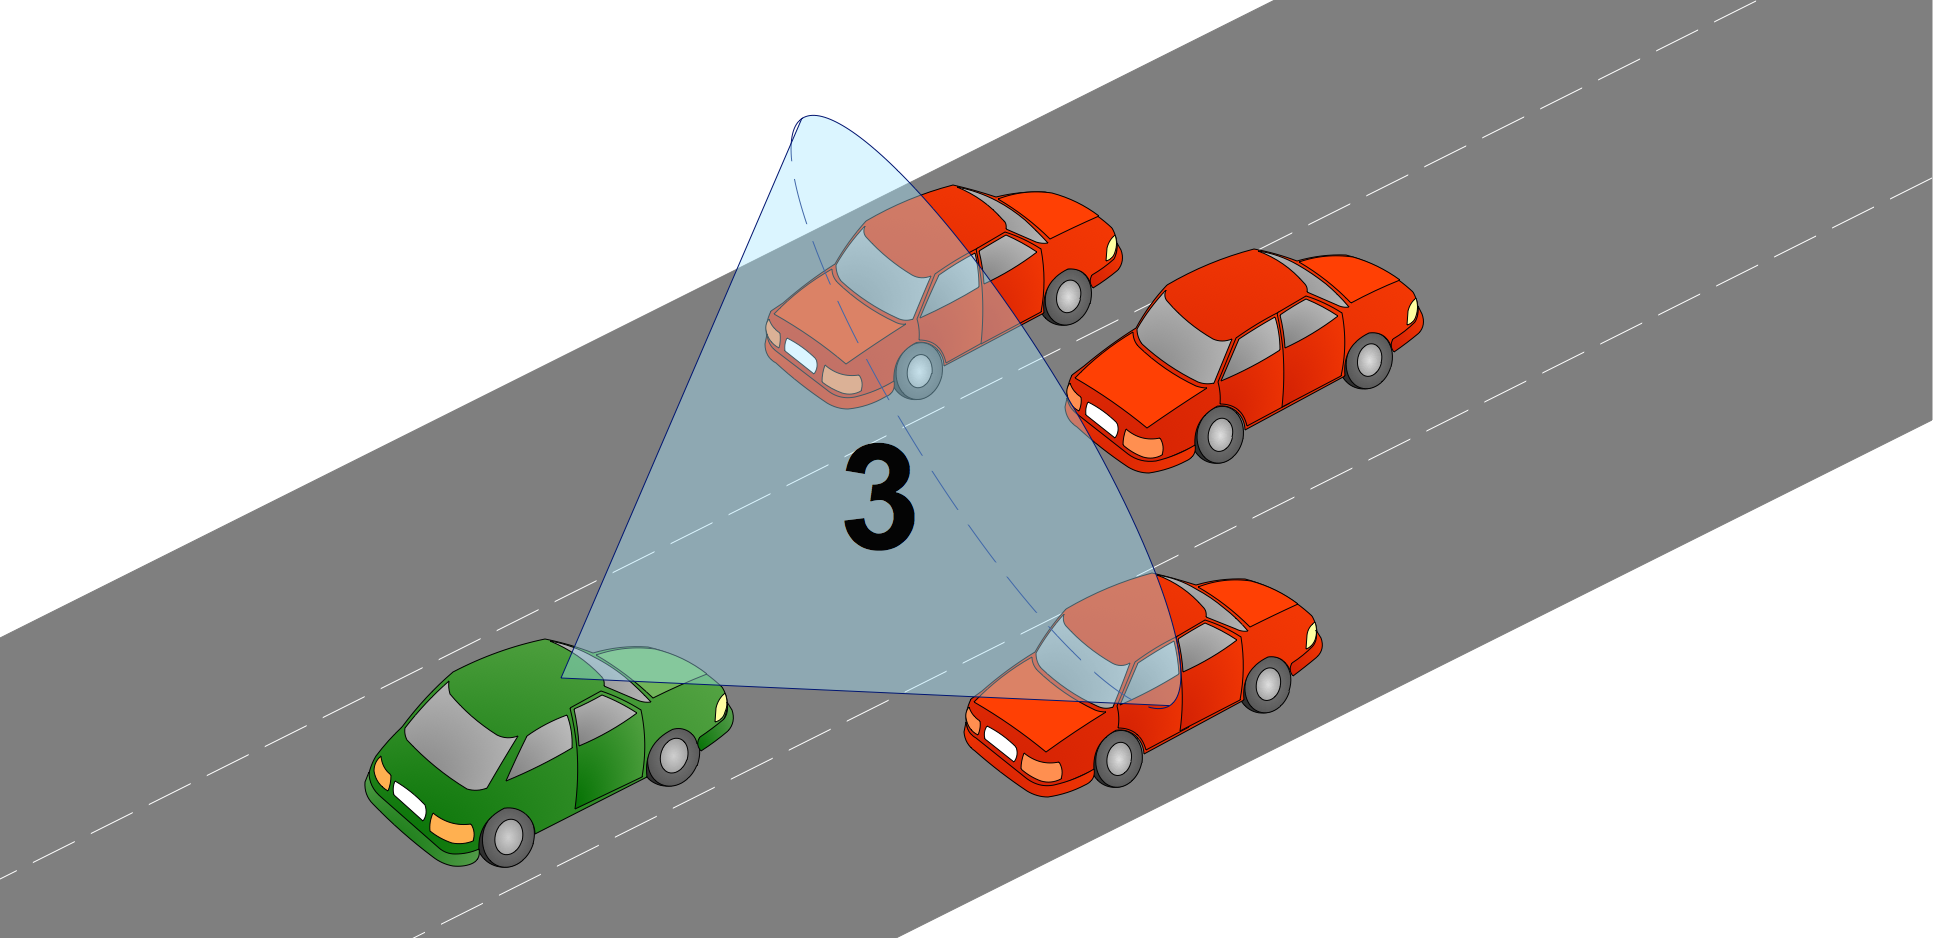
\includegraphics[width=0.28\textwidth]{text/figures/numOfObjects.png} \label{fig:introduction:semantics:a}} &
    \subfloat[\tiny{Distance to rear-end of vehicle directly in front.}]{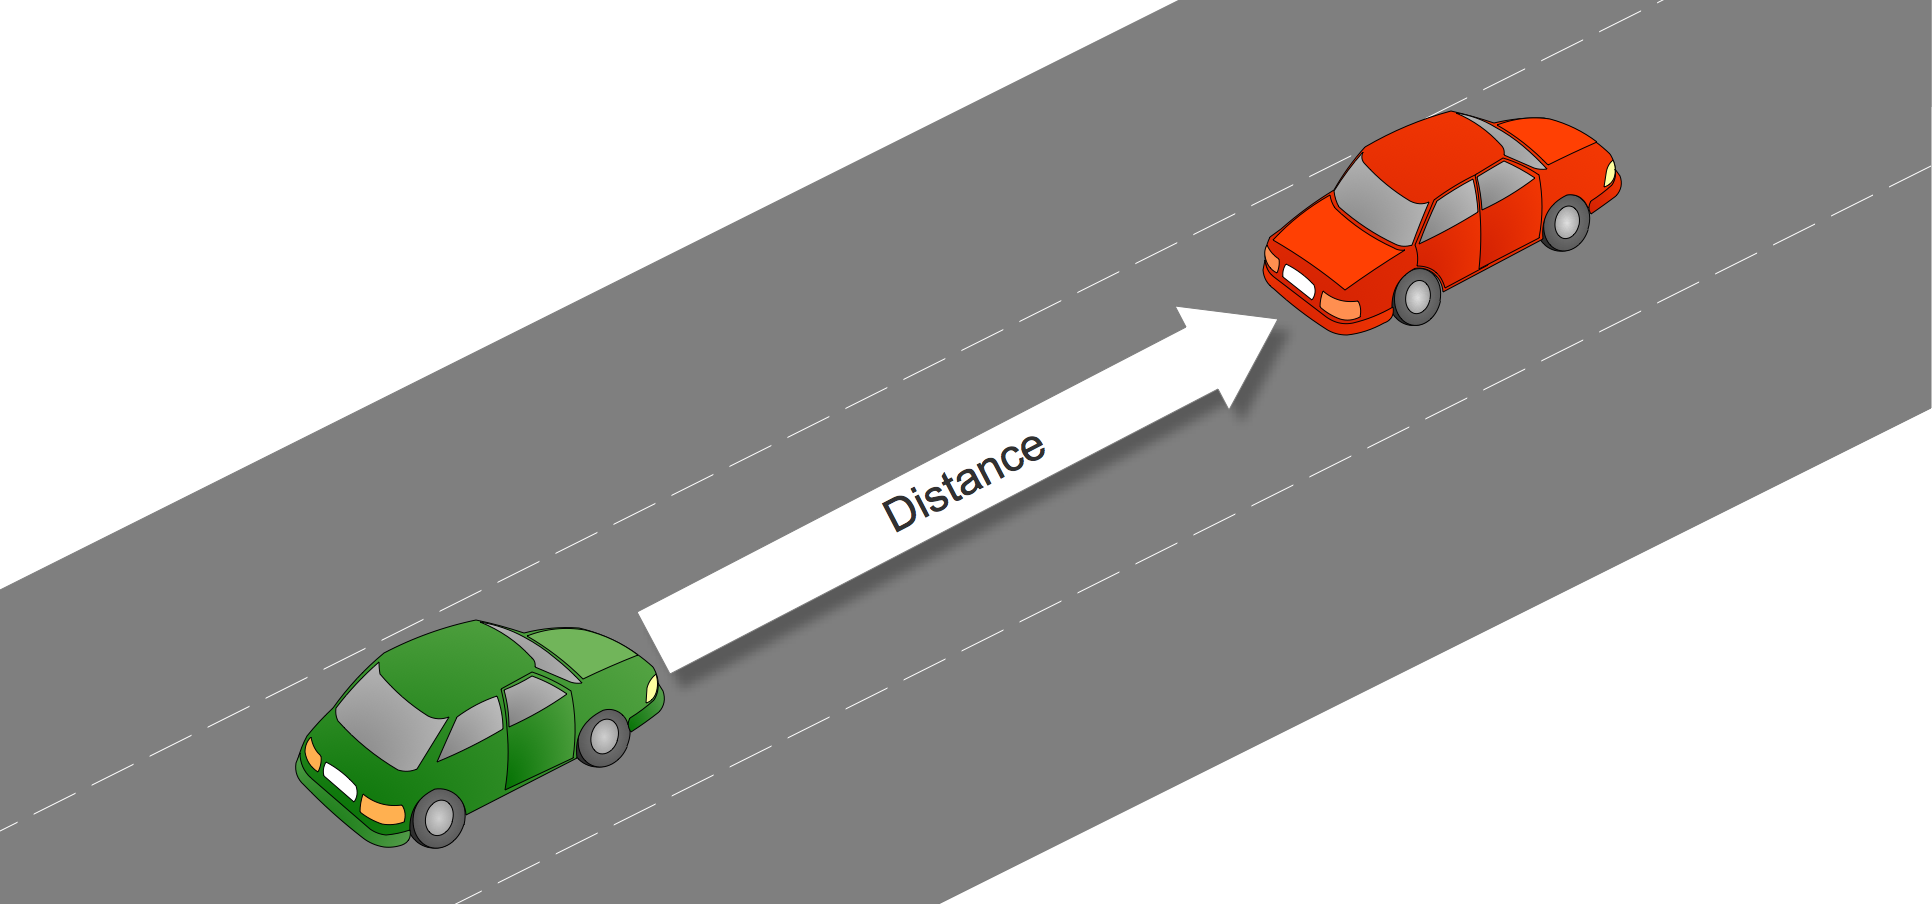
\includegraphics[width=0.28\textwidth]{text/figures/avgDistanceSameLane.png} \label{fig:introduction:semantics:b}} &
    
    \subfloat[\tiny{Other vehicle entering intersection - left turn across path.}]{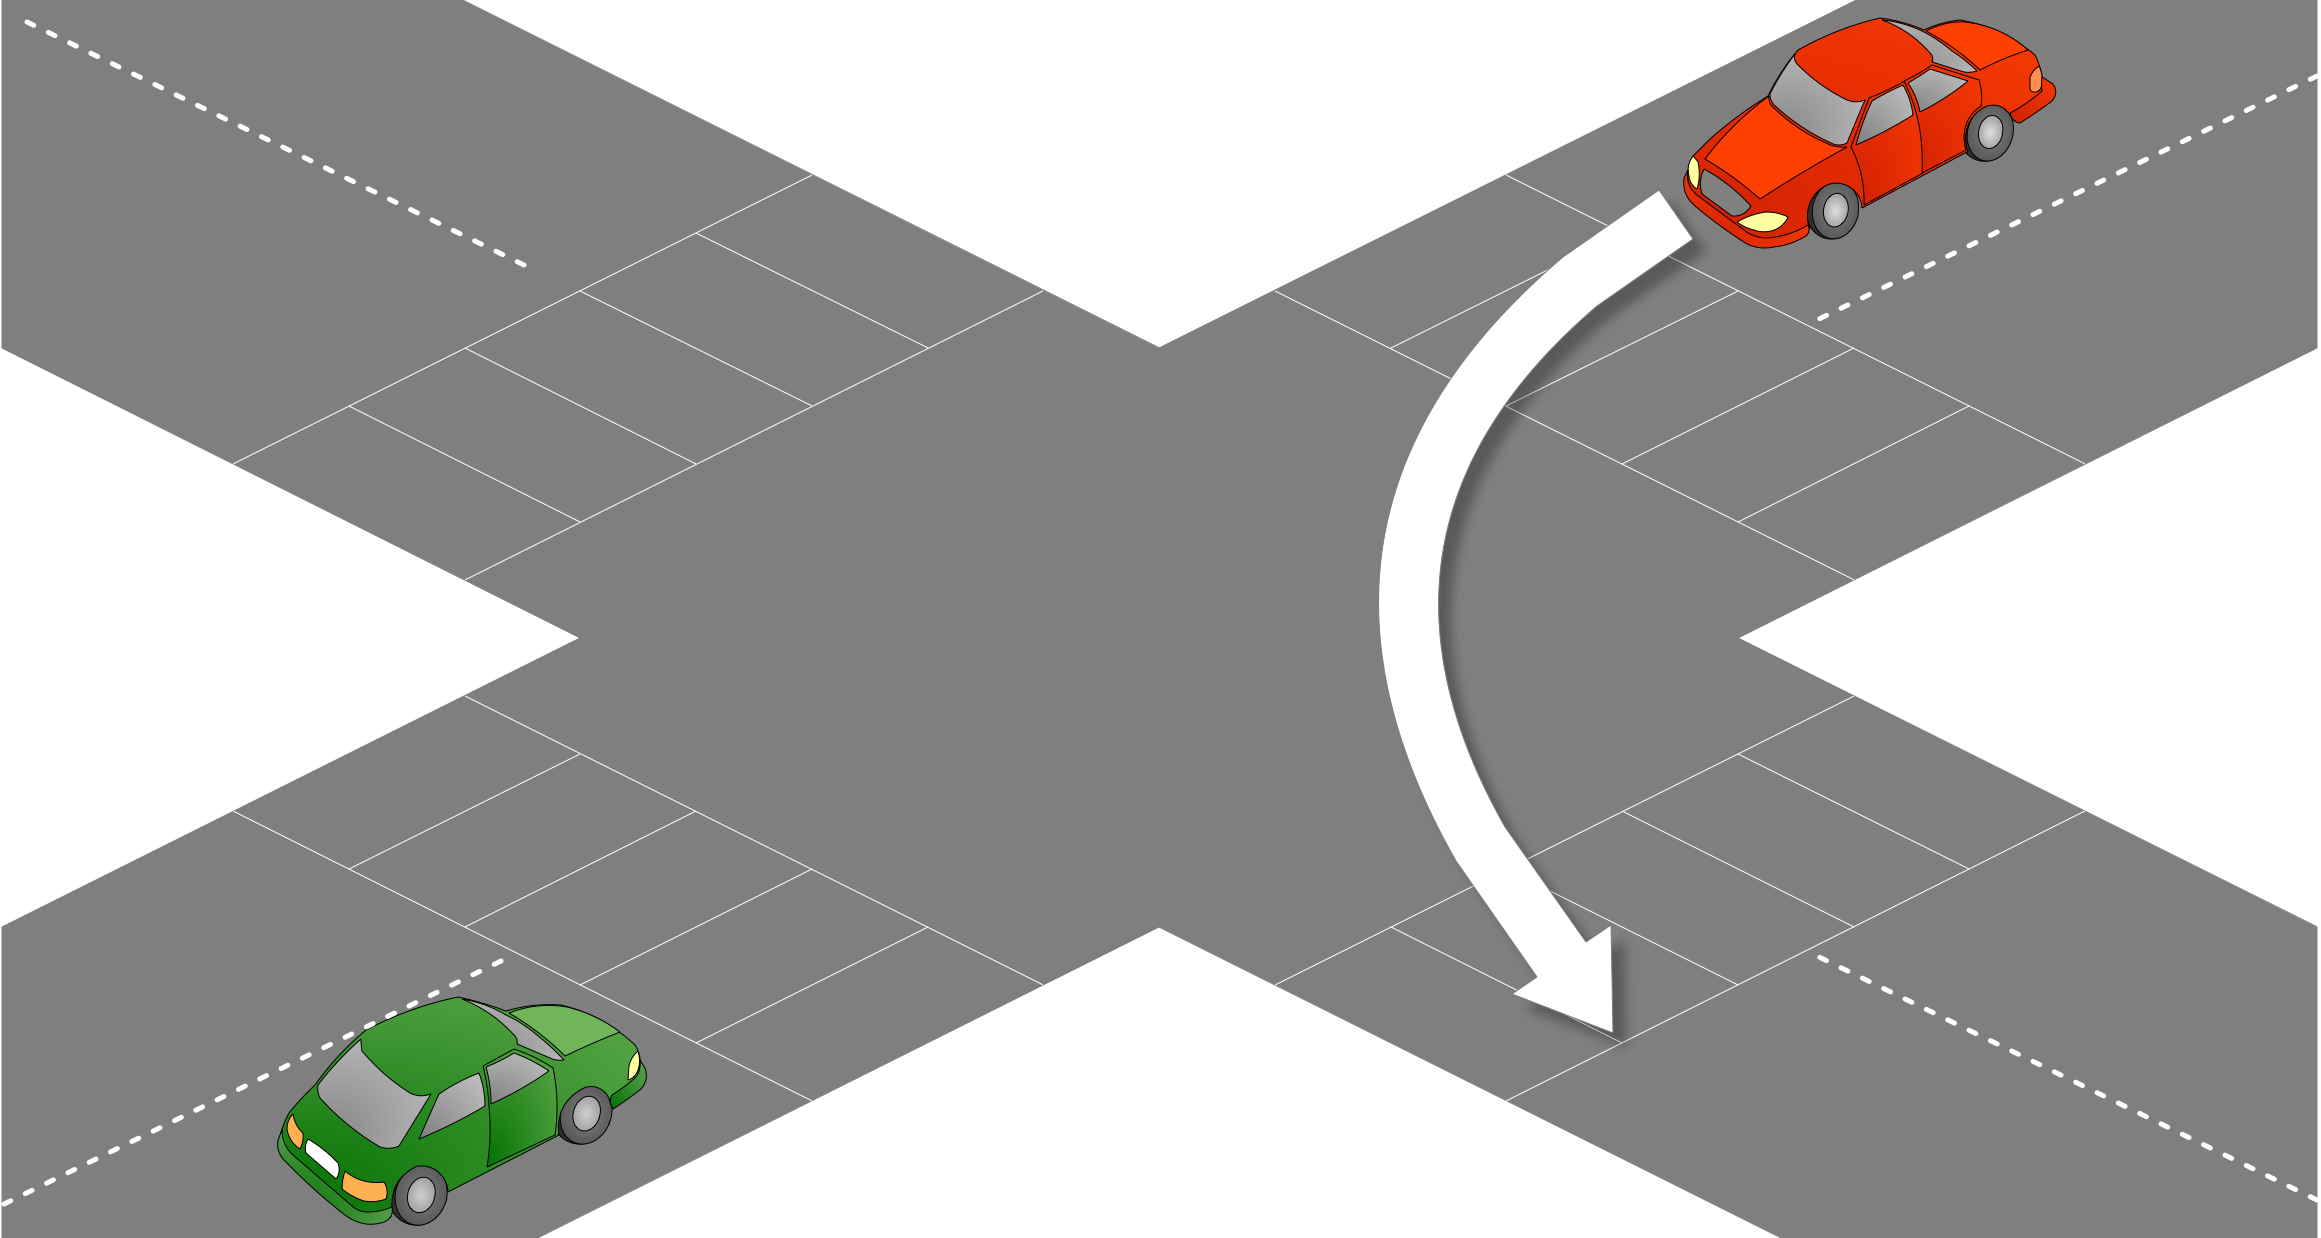
\includegraphics[width=0.28\textwidth]{text/figures/leftIntersect.png} \label{fig:introduction:semantics:c}} \\
    \subfloat[\tiny{Other vehicle entering intersection - turning onto opposite direction.}]{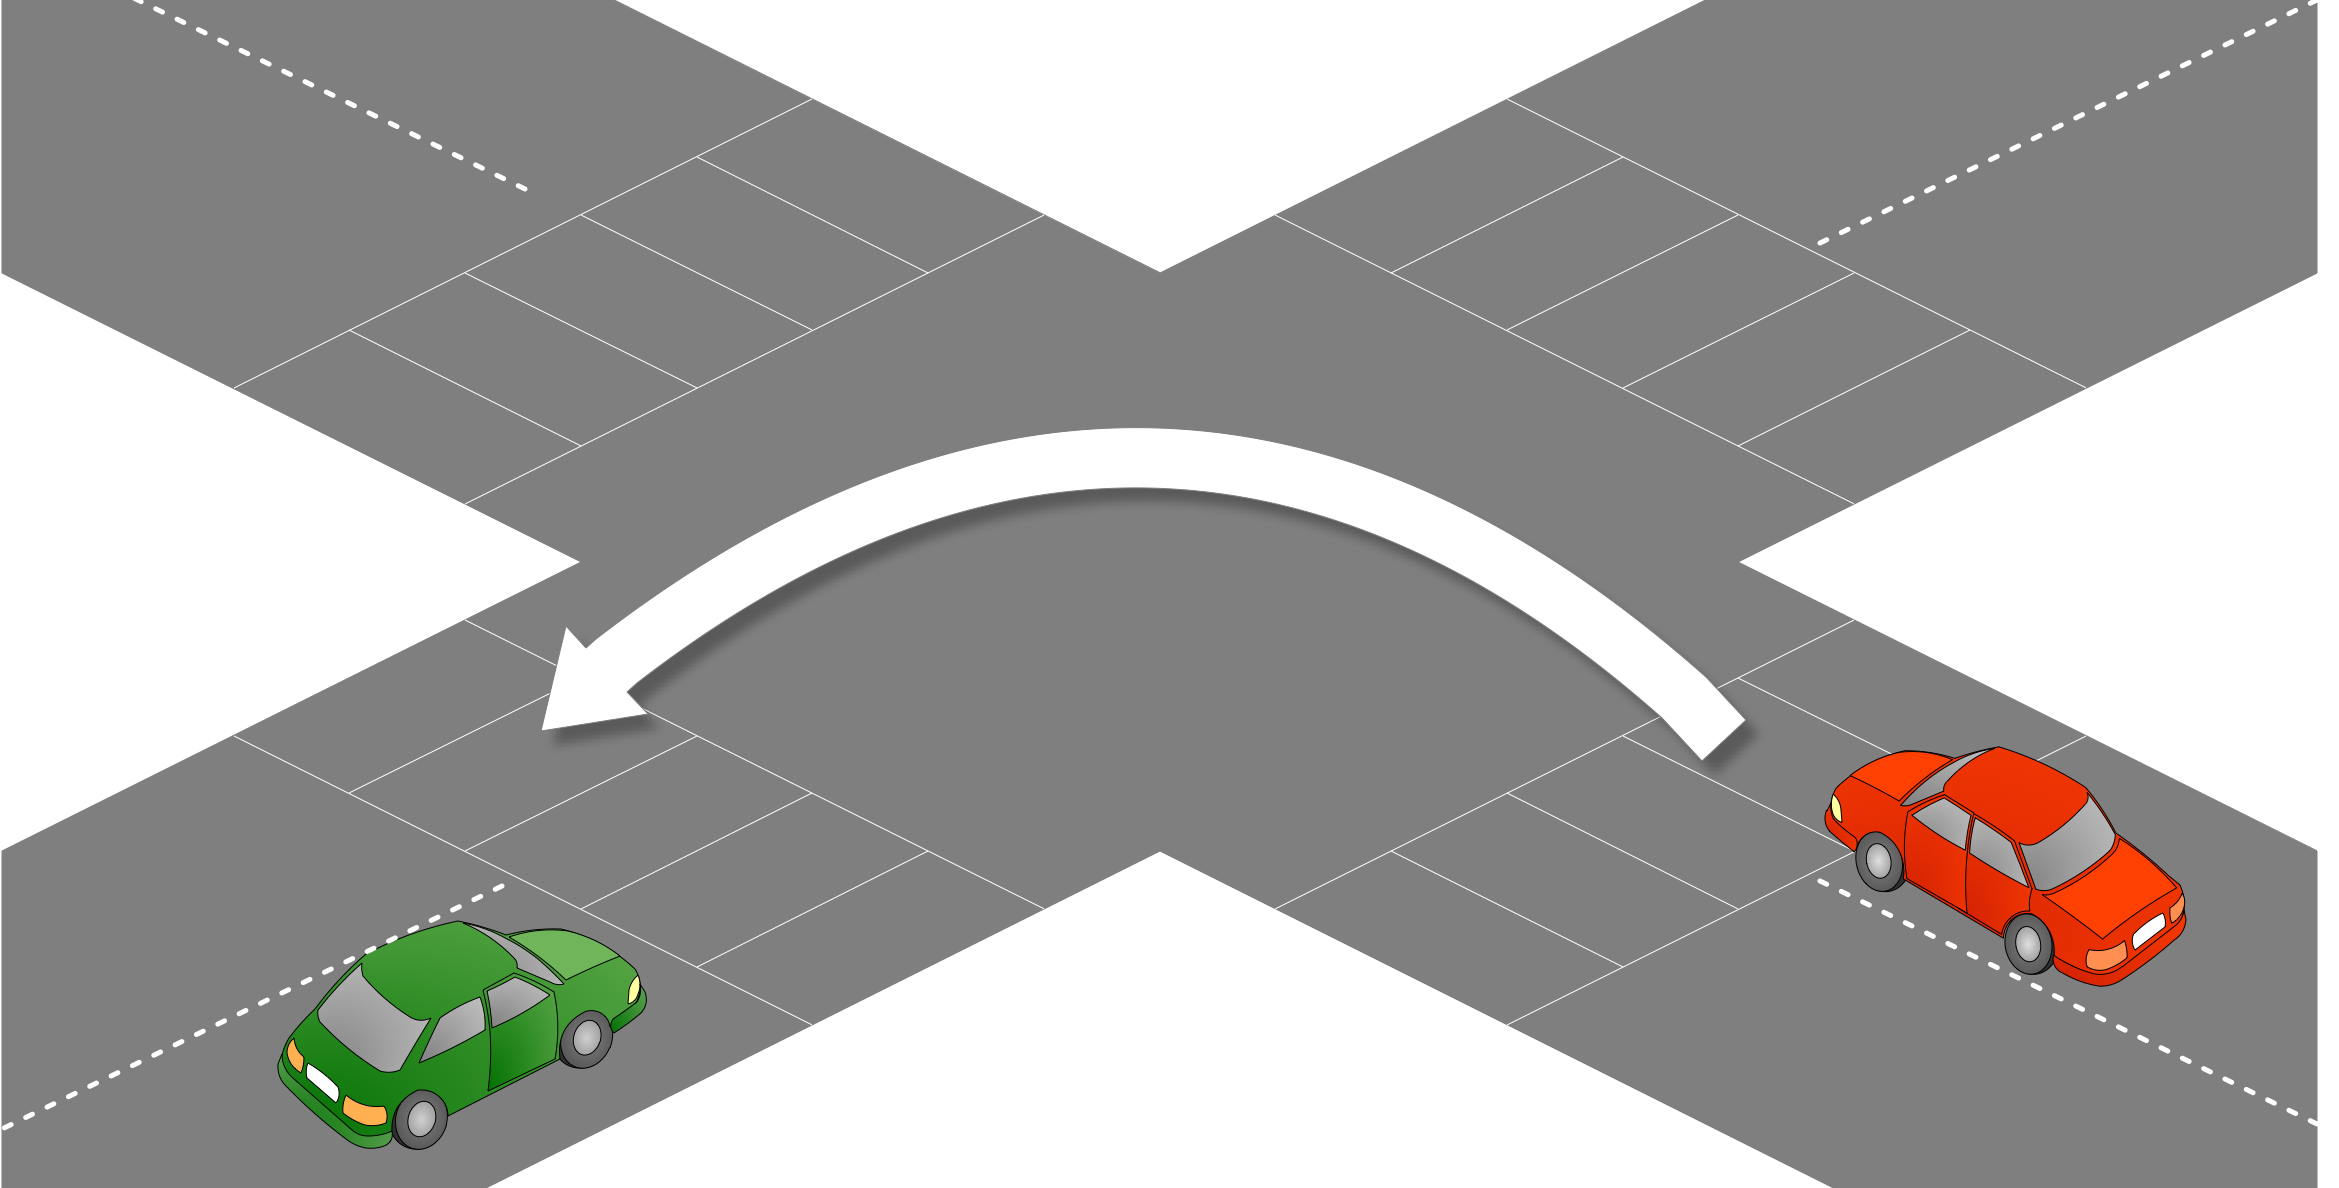
\includegraphics[width=0.28\textwidth]{text/figures/turningO.png} \label{fig:introduction:semantics:d}}&
    
    \subfloat[\tiny{Other vehicle entering intersection - straight across path.}]{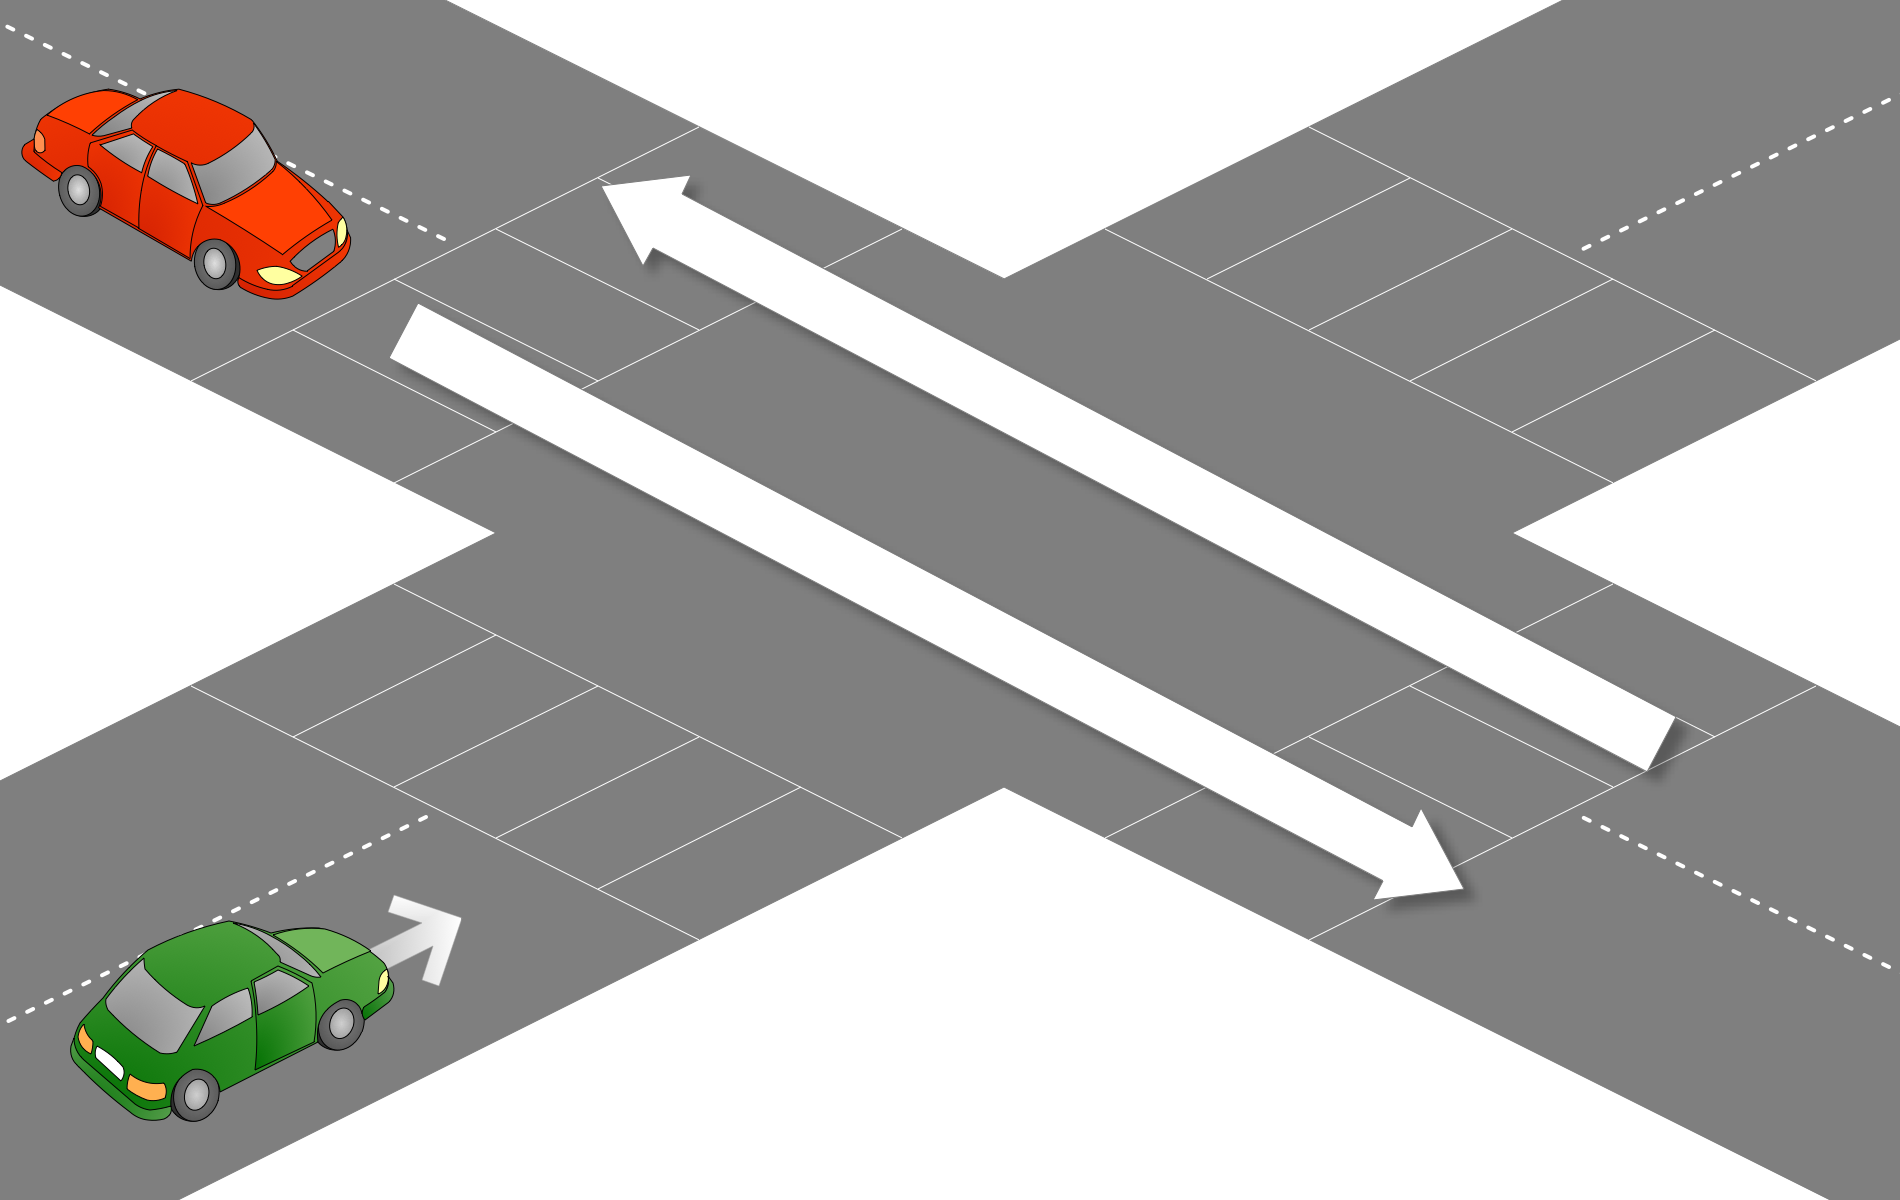
\includegraphics[width=0.28\textwidth]{text/figures/passingIntersect.png} \label{fig:introduction:semantics:e}} &
    \subfloat[\tiny{Other vehicle entering intersection - turning same direction.}]{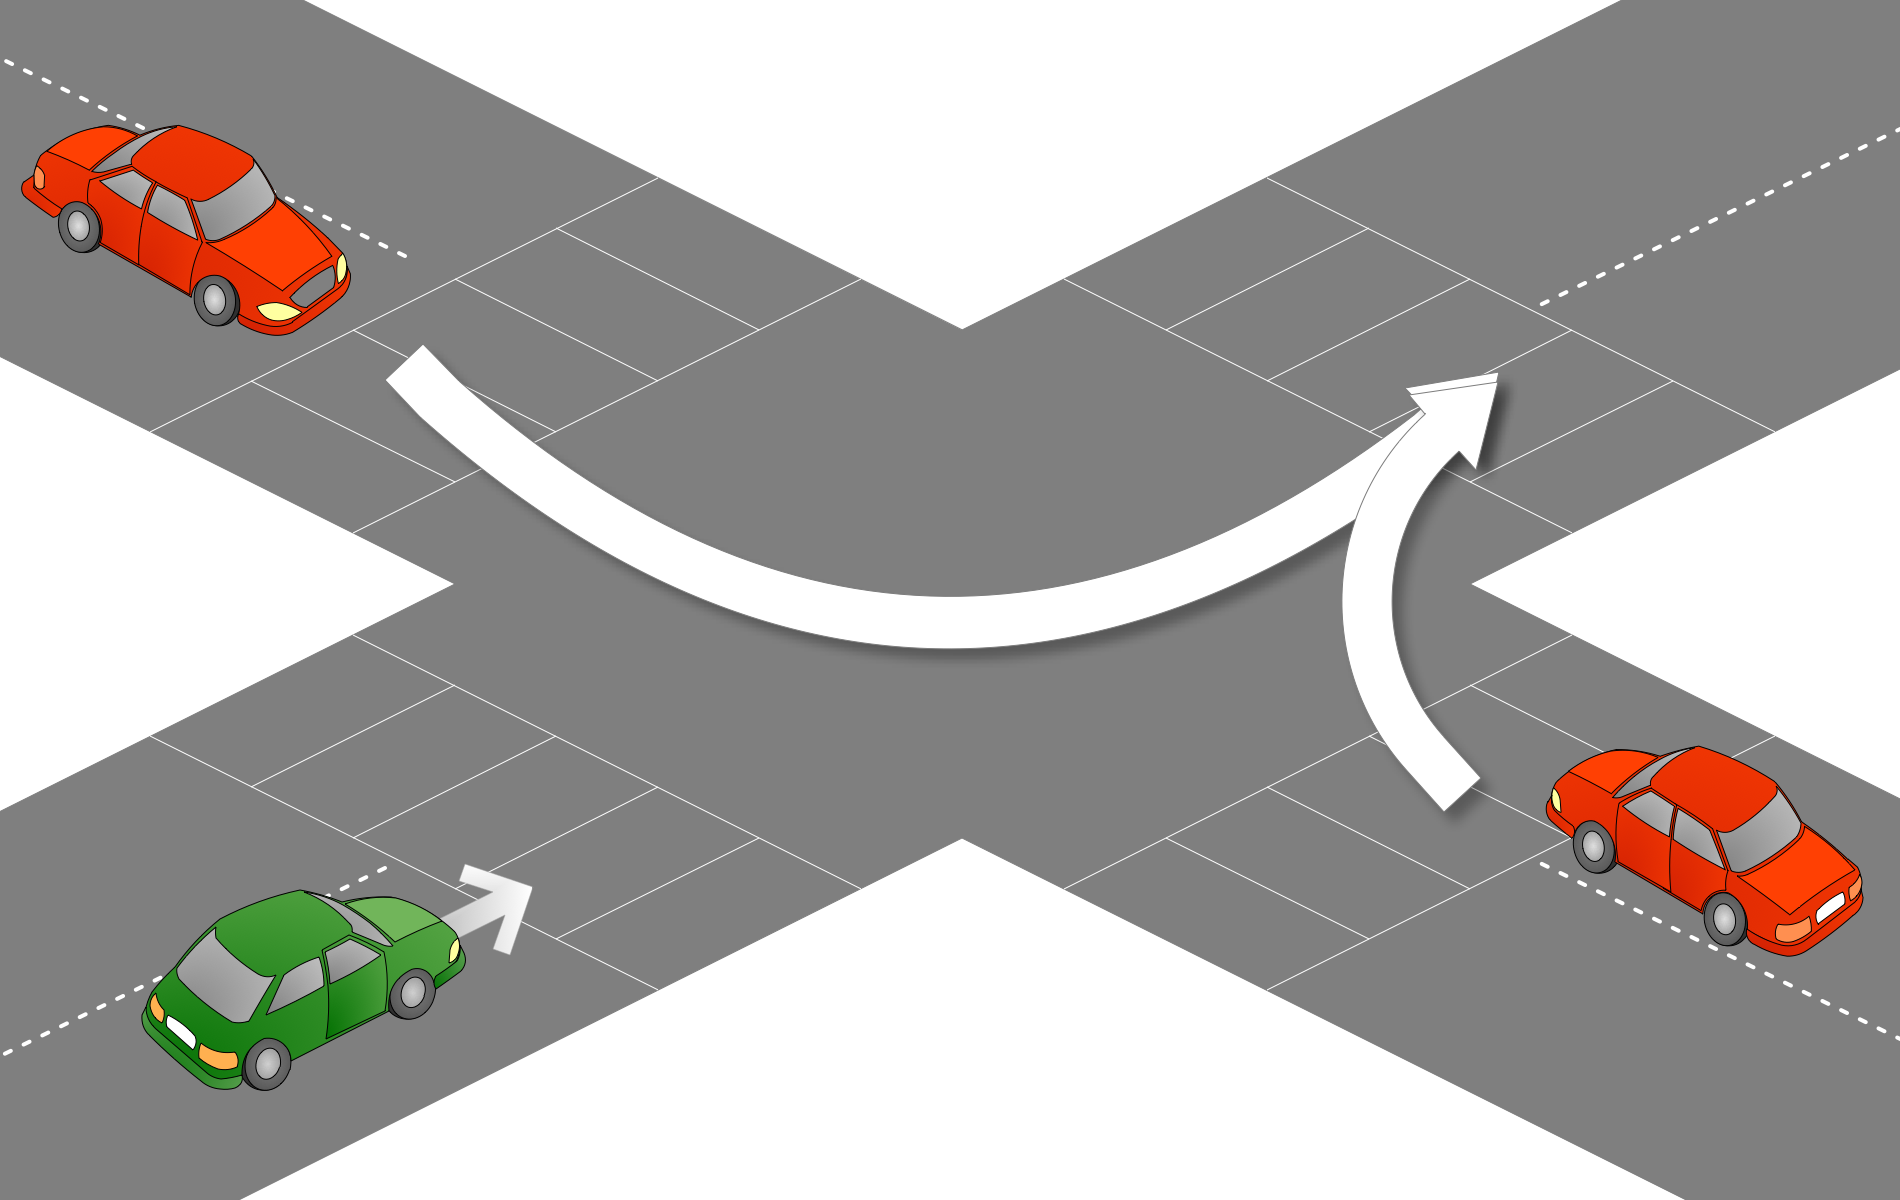
\includegraphics[width=0.28\textwidth]{text/figures/passingIntersectOntoSameDirection.png} \label{fig:introduction:semantics:f}}
  \end{tabular}
  \caption{\scriptsize{Critical events that can be automatically detected by the proposed method. Green car is ego vehicle. Red cars are other vehicles.\cite{philipsen2015NDS} } 
%(a) Average number of cars in front of ego-vehicle (b) Distance to rear-end of vehicle directly in front. (c) Other vehicle entering intersection - left turn across path (d) Other vehicle entering intersection - turning onto opposite direction (e) Other vehicle entering intersection - straight across path (f) Other vehicle entering intersection - turning same direction.
}
\label{fig:introduction:semantics}
\end{figure}

\vspace*{-3mm}
Our contributions are:
\begin{itemize}
\item Using stereo-vision for automatic event detection in both day and nighttime, with focus on intersections (Figure \ref{fig:introduction:semantics:c}, \ref{fig:introduction:semantics:d}, \ref{fig:introduction:semantics:e}, \ref{fig:introduction:semantics:f}).
\item Introducing a new event: Average number of vehicles in front of the ego vehicle. (Figure \ref{fig:introduction:semantics:a}).
\item Introducing a new event: Average distance to vehicles directly in front of the ego vehicle. (Figure \ref{fig:introduction:semantics:b}).
\end{itemize}

%\vspace{0.5pt}